\documentclass[12pt, letterpaper]{article}
\usepackage{iarc_latex_style}
\usepackage{amssymb,amsmath,listings,url,verbatim,graphicx}

\title{Beohawk: Autonomous Quadrotor}
\begin{document}
\maketitle
\begin{people}
\name{Rustom Jehangir}
\org{University of Southern California}
\name{Christopher Li}
\org{University of Southern California}
\end{people}

%1) Abstract	5
\begin{abstract}
	In this paper, we introduce a Micro UAV system that can explore an unknown indoor space without the assistance of a positioning system such as GPS. The robot takes in various kind of sensing measurements, handles them with probabilistic theories, and completes tasks such as stabilization and SLAM. \todo{Finish abstract at the end} (5 points)
\end{abstract}

%2) Introduction	5
%  a) Statement of the problem 
%  b) Conceptual solution to solve the problem
%    b1) Figure of overall system architecture 
%  c) Yearly Milestones
\section{Introduction}
The USC Aerial Robotics Team's \textit{Beohawk} quadrotor was designed to suit the requirements of the International Aerial Robotics Competition. The quadrotor uses a variety of sensors to measure and identify the environment it is in with the effort of searching for small object in a complex and unknown setting.

\subsection{Problem Statement}
For the sixth IARC mission, our quadrotor must navigate an unknown office environment to find a small flash drive, retrieve it, and return in under ten minutes while avoiding detection.  The vehicle, which weighs under 1.5kg, must also operate autonomously, which introduces the challenge of mapping and navigating an environment sensed with instruments that have random errors and noise. 

\subsection{Conceptual Solution}
The USC Aerial Robotics Team is implementing a solution based on a traditional approach to autonomous robotics with modifications for the mission and for the mechanics of the robot. The quadrotor is custom built to be within the required weight and size range and uses a commercial control board for low level control. An onboard computer uses the Robotic Operating System (ROS) and takes advantage of many of the packages and tools made available by public contributors. 

\subsubsection{Figure of Overall System Architecture}

Figure \eqref{fig:architecture} shows the basic system architecture of the quadrotor. The quadrotor's low level control including stability, attitude control, altitude control, and position control are all performed by the low-level control board. This board is an Arduino based board that has sensors and motor outputs. It also receives radio-control signals and allows control to be over-ridden by a human pilot.

The main computer is a Pico-ITX form-factor x86 based computer that handles higher level control. This computer runs ROS, which performs optical flow calculations for basic positional stability. \sout{This computer also runs the navigator that decides where the robot will move and what actions it will take. More computationally expensive processes such as SLAM, take place on an off-board computer with a more powerful processor and more memory.} Mission planning, navigation, and SLAM take place on the base station, which has a more powerful processor and more memory. The quadrotor publishes sensor data and subscribes to navigation positions from the base station.

\begin{figure}[h]
\centering
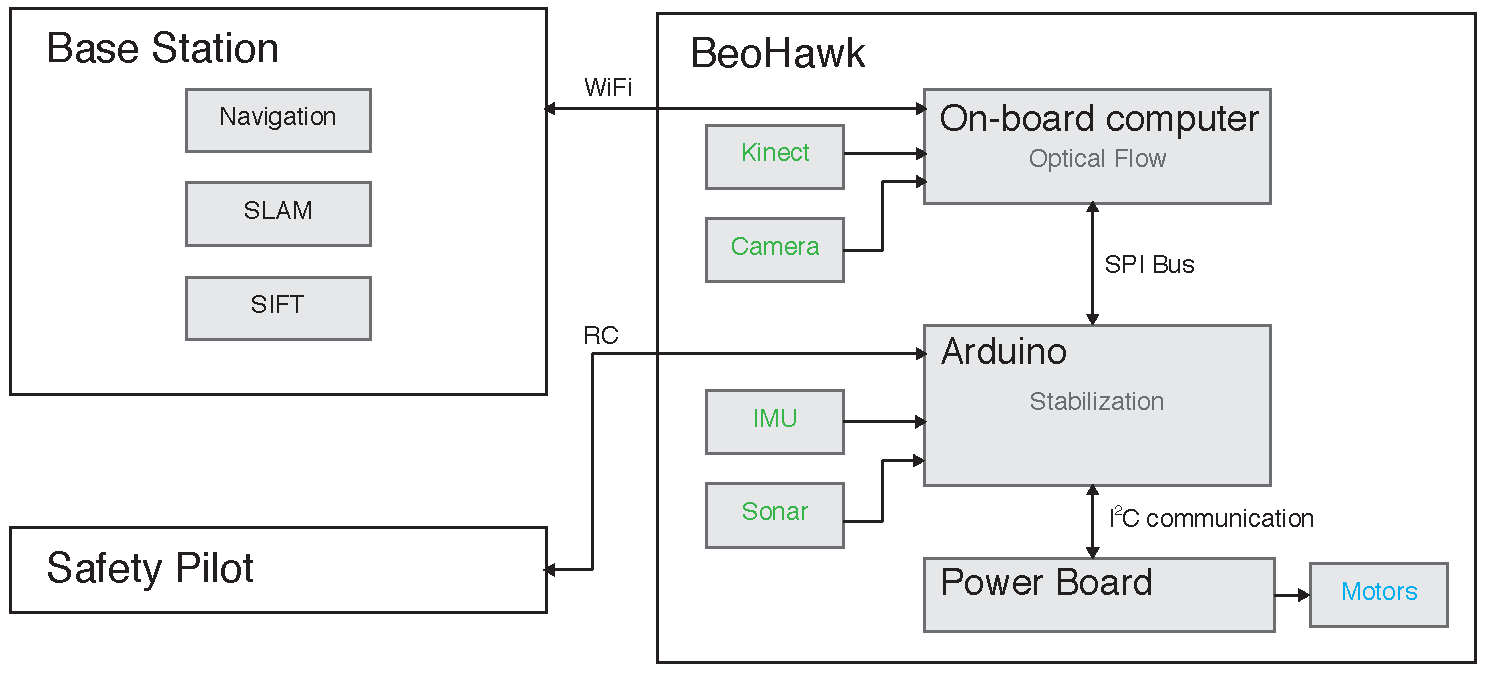
\includegraphics[width=14cm]{images/beohawk-system-arch.pdf}
\caption{General architecture of the Beohawk control system. \todo{This needs to be completed}.} 
\label{fig:architecture}
\end{figure}

\subsection{Yearly Milestones}
This is USC's first appearance at the IARC and our team's first competition. This year we hope to develop a platform capable of mapping and navigating the environment.  If we do not complete the goals, we will continue refining the quadrotor. \todo{eh.. feels lacking}

%3) Air Vehicle	15
%  a) Propulsion and Lift System 
%  b) Guidance, Nav., and Control 
%    b1) Stability Augmentation System 
%    b2) Navigation 
%    b3) Figure of control system architecture 
%  c) Flight Termination System
\section{Air Vehicle}

\subsection{Propulsion and Lift System}
\emph{Beohawk} has four rotors, each an equal distance from the quadrotor's center.  Two opposite motors spin clockwise and the other two spin counter-clockwise, which generates a net torque of zero.  Hence, the quadrotor does not need a separate rotor to control yaw like a conventional helicopter, and can control yaw by adjusting the proportion of rotor speeds.  \todo{Todo: More details on these rotors}

\subsection{Guidance, Navigation, and Control}

\subsubsection{Stability Augmentation System}
Beohawk stabilizes itself through a control loop instead of relying on mechanical stability. 
\todo{Something about stability}
Center: carbon fiber
standoffs: alu
motor arms: carbon fiber

\begin{figure}[h]
\centering
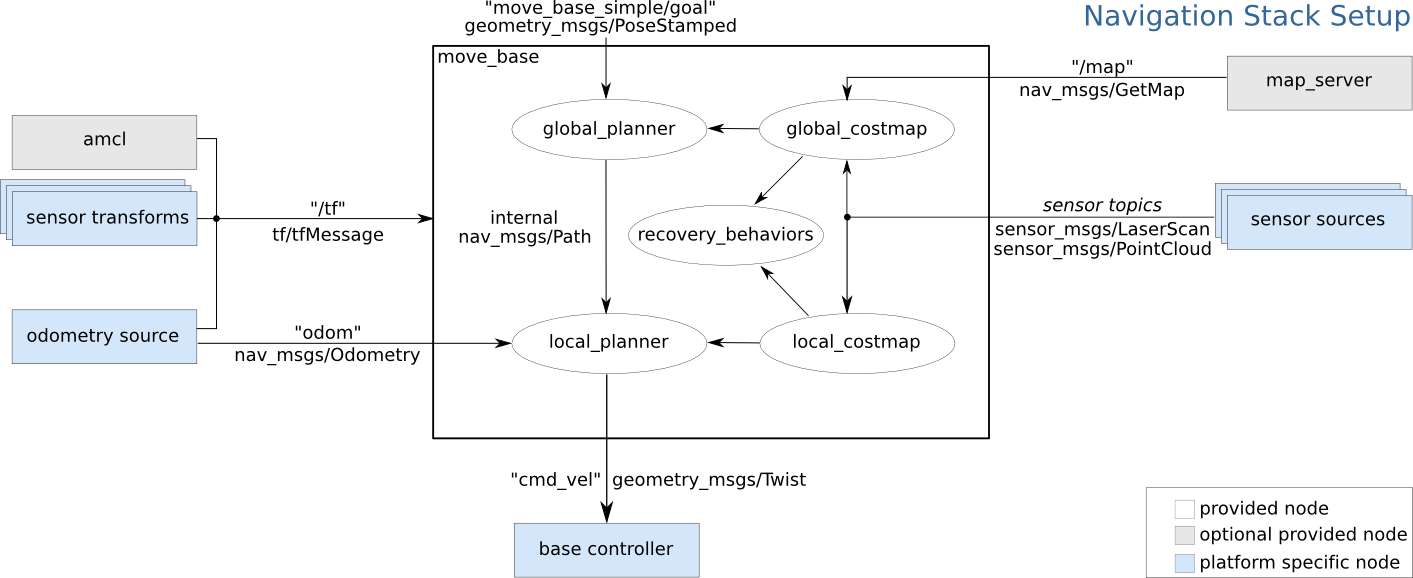
\includegraphics[width=12cm]{images/overview_tf.png}
\caption{Navigation system of Beohawk. \todo{This is a placeholder}.} 
\label{fig:navi}
\end{figure}

\subsubsection{Navigation}
Navigation is done in 2D using the navigation ROS package. Figure \eqref{fig:navi} shows the inputs to the navigation stack. Mission control is managed with a state machine that keeps track of the current objective.  \todo{Possibly a state diagram? To finish later}


\subsubsection{Figure of Control System Architecture}

\begin{figure}[h]
\centering
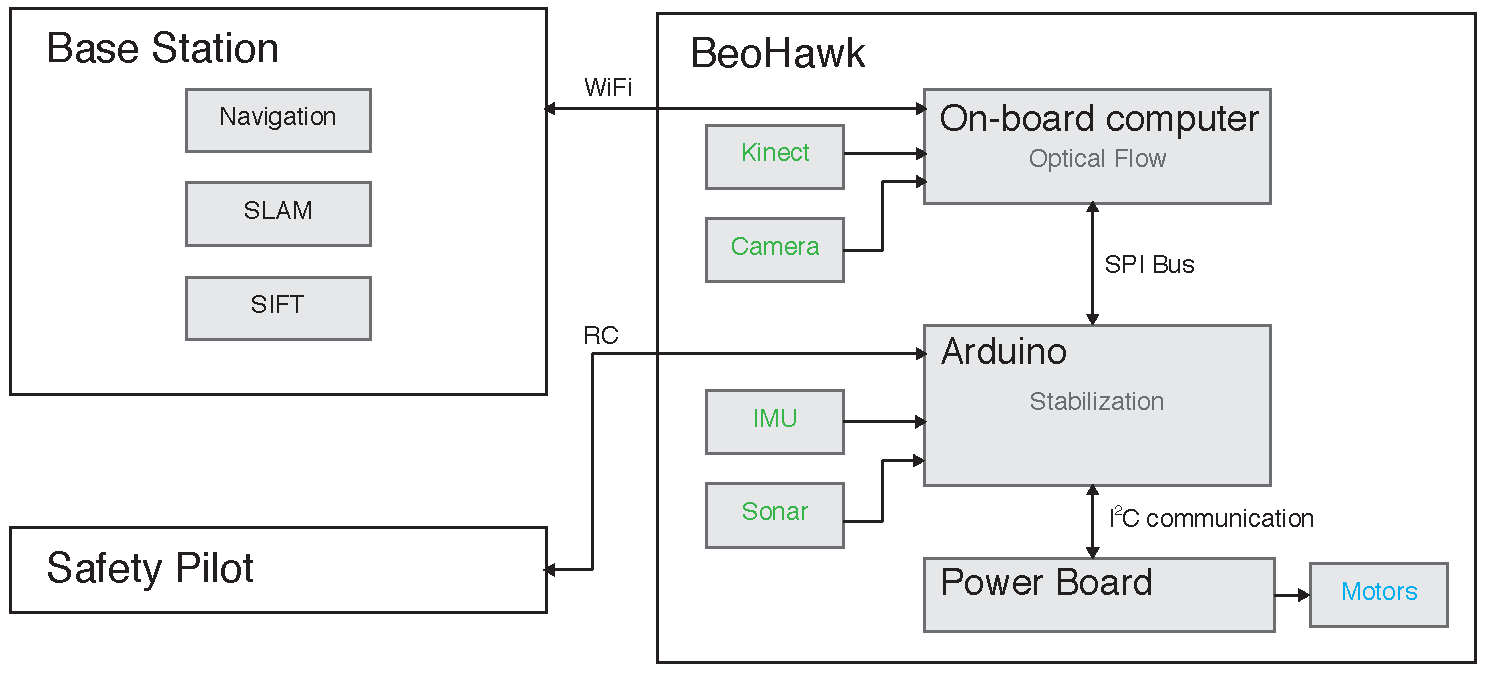
\includegraphics[width=14cm]{images/beohawk-system-arch.pdf}
\caption{Control system architecture. \todo{This needs to be completed}.} 
\label{fig:architecture}
\end{figure}

\todo{And an explanation}

\subsection{Flight Termination System}
Because the RC controller communicates directly with the Arduino, the safety pilot can terminate the operation of the quadrotor in the event it is needed.

%4) Payload	15
%  a) Sensor Suite 
%    a1) GNC Sensors 
%    a2) Mission Sensors 
%      a21) Target Identification 
%      a22) Threat Avoidance 
%  b) Communications 
%  c) Power Management System 
%  d) Sub-Vehicle (if any)
\section{Payload}
\subsection{Sensor Suite}
\subsubsection{Microsoft Kinect}
The Kinect uses an infrared laser array of 640x480 points to provide depth information at 2048 levels of sensitivity. Beohawk points the Kinect sensor down at a 45$^\circ$ angle.  A ROS package uses the Kinect to produce a point cloud, which gives Beohawk a plane of vision with depth information.  Within this point cloud, there should be a kink where the floor is.  This allows us to estimate altitude.  We detect walls in a similar fashion, so that we can avoid colliding with the wall.

\subsubsection{Camera}
Using a downward facing camera, the quadrotor runs an optical flow algorithm on the x86 processor to reduce drift.  A second, front-facing camera captures pictures for reading the signs above the doors.  The images are published through the wireless network to the base station, which runs SIFT to detect the Chief of Security's office via the sign above the door. The front camera is also responsible for detecting the blue security light.  The bottom camera is used to identify the flash drive.

\subsubsection{Sonar}
Though the quadrotor has an estimate of altitude from the Kinect, it may be noisy and as such, the quadrotor also employs sonar to determine altitude.  A \todo{model/part number} is installed facing downwards.

\subsubsection{Target Identification}
\todo{Reading signs}

\subsubsection{Threat Avoidance}
\todo{How will we dodge the laser tripwires?}

\subsection{Communications}
The Pico-ITX computer aboard the quadrotor communicates with the Arduino over an SPI bus running at \todo{n} Hz.  It also communicates with the base station over a 2.4GHz wifi link.  The communication rate varies by sensor topic. The Pico publishes the Kinect point cloud at \todo{n} Hz, the camera images at \todo{n} Hz, and the vehicle status and battery info at \todo{n} Hz.

The Arduino communicates with the power board with I$^2$C at \todo{n} Hz. It also connects to an RC control device that operates at \todo{n} GHz.

\subsection{Power Management System}
Beohawk is powered by a 7.4V 500mAh Lithium-Polymer battery pack, which provides enough energy to run at least ten minutes. A power regulator board controls the battery and motor speed.  In the event of low power, the base station initiates a controlled descent to avoid damage to the quadrotor. 

%5) Operations	10
%  a) Flight Preparations 
%    a1) Checklist(s) 
%  b) Man/Machine Interface
\section{Operations}

\subsection{Flight Preparations}
Before any flight is performed, batteries must be charged an an able human operator must be available to assume the control the RC controller.  For competition, the following checklist must be completed.

\subsubsection{Competition Checklist}
\begin{enumerate}
  \item Inspect and test hardware
  \item Launch ROS nodes
  \item Check software status
  \item Ensure RC link works
  \item Test hover in place
  \item Start mission control
\end{enumerate}

\subsection{Man-Machine Interface}
The base station displays Beohawk's current mission and status inferred from the sensor data returned by Beohawk.  If the link is terminated, Beohawk will  hover in place until the connection is restored or until the human operator assumes control. The human operator has an RC controller that communicates directly with the Arduino.


%6) Risk Reduction	15
%  a) Vehicle Status 
%    a1) Shock/Vibration Isolation 
%    a2) EMI/RFI Solutions 
%  b) Safety 
%  c) Modeling and Simulation 
%  d) Testing
\section{Risk Reduction}
\subsection{Vehicle Status}
Beohawk transmits battery information, sensor information, and current objective to the base station. 

\subsubsection{Shock/Vibration Isolation}
\todo{Keith has some stuff on this}

\subsubsection{EMI/RFI Solutions}
Because our sensors and electronics are not very sensitive to the interference from motors and wireless communications, we have not had to worry about EMI or RFI.

\subsection{Safety}

\subsection{Modeling and Simulation}
Hardware was modeled in SolidWorks.

\subsection{Testing}
We have done continuous testing on Beohawk as we developed it. \todo{hardware testing methodology}

For software, we did field tests to ensure the proper functioning of SLAM and vision algorithms.  SLAM was prototyped in MATLAB and re-written in C++ while the mission control was written in Python and has a unit test suite as well as a behavior test suite. 

\begin{table}[h]
\centering
\begin{tabular}{l  r  r  r}
                                       & Used  & Avail. & Perc. \\
  Number of Slices:                    &  684  & 4656  &  14\%  \\
  Number of Slice Flip Flops:          &  198  & 9312  &   2\%  \\
  Number of 4 input LUTs:              & 1316  & 9312  &  14\%  \\
  Number of IOs:                       &   37  &       &      \\
  Number of bonded IOBs:               &   36  &  232  &  15\%  \\
  Number of BRAMs:                     &    2  &   20  &  10\%  \\
  Number of MULT18X18SIOs:             &   10  &   20  &  50\%  \\
  Number of GCLKs:                     &    2  &   24  &   8\%  \\
\end{tabular}
\caption{Resource usage.}
\label{tab:usage}
\end{table}


%7) Conclusion	5 
\section{Conclusion (5)}
Use tables and figures to concisely state your point. A table title appears above the table it references and appears in all caps and centered, whereas a figure title appears beneath the figure and with only leading capitalization. Both table and figure titles are italicized as shown in the examples below:


%8) References	5
\bibliographystyle{IEEEbib}
\begin{thebibliography}{10}
\bibitem[1]{bib:kinectinfo} \url{http://git.marcansoft.com/?p=libfreenect.git;a=summary/}
\end{thebibliography}


\end{document}